% This file is generated by the MATLAB m-file laprint.m. It can be included
% into LaTeX documents using the packages graphicx, color and psfrag.
% It is accompanied by a postscript file. A sample LaTeX file is:
%    \documentclass{article}\usepackage{graphicx,color,psfrag}
%    \begin{document}% This file is generated by the MATLAB m-file laprint.m. It can be included
% into LaTeX documents using the packages graphicx, color and psfrag.
% It is accompanied by a postscript file. A sample LaTeX file is:
%    \documentclass{article}\usepackage{graphicx,color,psfrag}
%    \begin{document}% This file is generated by the MATLAB m-file laprint.m. It can be included
% into LaTeX documents using the packages graphicx, color and psfrag.
% It is accompanied by a postscript file. A sample LaTeX file is:
%    \documentclass{article}\usepackage{graphicx,color,psfrag}
%    \begin{document}% This file is generated by the MATLAB m-file laprint.m. It can be included
% into LaTeX documents using the packages graphicx, color and psfrag.
% It is accompanied by a postscript file. A sample LaTeX file is:
%    \documentclass{article}\usepackage{graphicx,color,psfrag}
%    \begin{document}\input{f_Qs_30_p_5_1}\end{document}
% See http://www.mathworks.de/matlabcentral/fileexchange/loadFile.do?objectId=4638
% for recent versions of laprint.m.
%
% created by:           LaPrint version 3.16 (13.9.2004)
% created on:           12-Nov-2008 21:46:31
% eps bounding box:     17.5 cm x 13.125 cm
% comment:              
%
\begin{psfrags}%
\psfragscanon%
%
% text strings:
\psfrag{s05}[b][b]{$\xi_{5}$}%
\psfrag{s06}[b][b]{$\xi_{25}$}%
\psfrag{s07}[b][b]{$\xi_{35}$}%
\psfrag{s08}[t][t]{$\nu$}%
\psfrag{s09}[b][b]{$\xi_{\nu}$}%
\psfrag{s10}[t][t]{Slot number}%
\psfrag{s11}[b][b]{$F_{slot}/\SI{}{A}$}%
%
% xticklabels:
\psfrag{x01}[t][t]{0}%
\psfrag{x02}[t][t]{5}%
\psfrag{x03}[t][t]{10}%
\psfrag{x04}[t][t]{15}%
\psfrag{x05}[t][t]{20}%
\psfrag{x06}[t][t]{25}%
\psfrag{x07}[t][t]{30}%
\psfrag{x08}[t][t]{0}%
\psfrag{x09}[t][t]{10}%
\psfrag{x10}[t][t]{20}%
\psfrag{x11}[t][t]{30}%
\psfrag{x12}[t][t]{40}%
\psfrag{x13}[t][t]{50}%
\psfrag{x14}[t][t]{60}%
%
% yticklabels:
\psfrag{v01}[r][r]{-1}%
\psfrag{v02}[r][r]{-0.5}%
\psfrag{v03}[r][r]{0}%
\psfrag{v04}[r][r]{0.5}%
\psfrag{v05}[r][r]{1}%
\psfrag{v06}[r][r]{0}%
\psfrag{v07}[r][r]{0.1}%
\psfrag{v08}[r][r]{0.2}%
\psfrag{v09}[r][r]{0.3}%
\psfrag{v10}[r][r]{0.4}%
\psfrag{v11}[r][r]{0.5}%
\psfrag{v12}[r][r]{0.6}%
\psfrag{v13}[r][r]{0.7}%
\psfrag{v14}[r][r]{0.8}%
\psfrag{v15}[r][r]{0.9}%
\psfrag{v16}[r][r]{1}%
\psfrag{v17}[r][r]{1.1}%
%
% Figure:

\subfloat[Slot mmf and winding factors\label{fig:f_Qs30_5_1}]{%
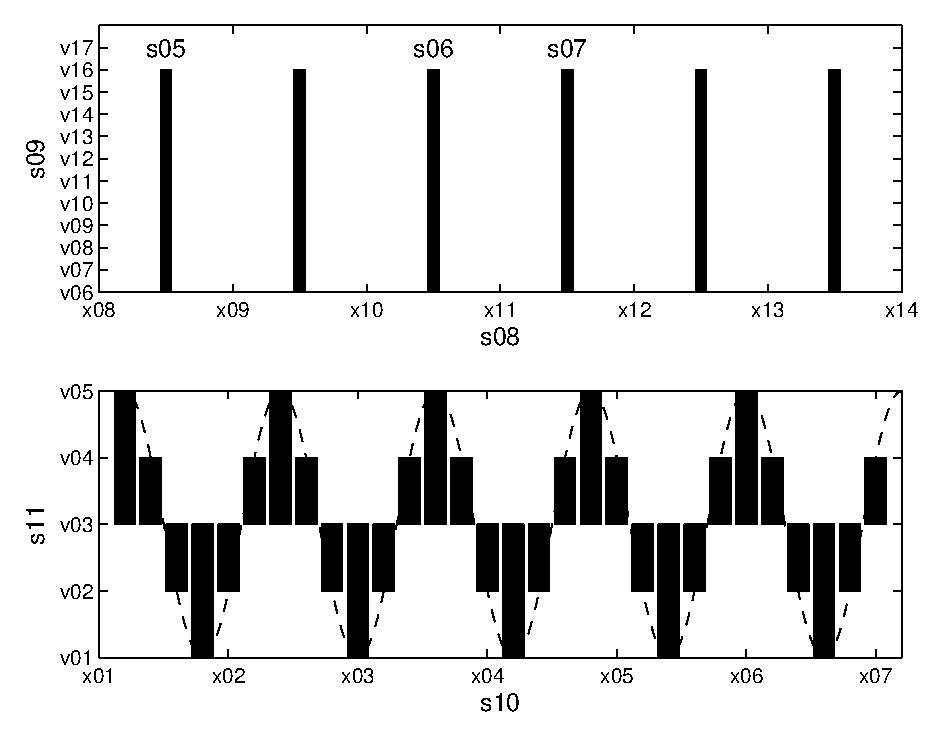
\includegraphics[width=0.9\textwidth]{figs/f_Qs_30_p_5_1.eps}}%
\end{psfrags}%
%
% End f_Qs_30_p_5_1.tex
\end{document}
% See http://www.mathworks.de/matlabcentral/fileexchange/loadFile.do?objectId=4638
% for recent versions of laprint.m.
%
% created by:           LaPrint version 3.16 (13.9.2004)
% created on:           12-Nov-2008 21:46:31
% eps bounding box:     17.5 cm x 13.125 cm
% comment:              
%
\begin{psfrags}%
\psfragscanon%
%
% text strings:
\psfrag{s05}[b][b]{$\xi_{5}$}%
\psfrag{s06}[b][b]{$\xi_{25}$}%
\psfrag{s07}[b][b]{$\xi_{35}$}%
\psfrag{s08}[t][t]{$\nu$}%
\psfrag{s09}[b][b]{$\xi_{\nu}$}%
\psfrag{s10}[t][t]{Slot number}%
\psfrag{s11}[b][b]{$F_{slot}/\SI{}{A}$}%
%
% xticklabels:
\psfrag{x01}[t][t]{0}%
\psfrag{x02}[t][t]{5}%
\psfrag{x03}[t][t]{10}%
\psfrag{x04}[t][t]{15}%
\psfrag{x05}[t][t]{20}%
\psfrag{x06}[t][t]{25}%
\psfrag{x07}[t][t]{30}%
\psfrag{x08}[t][t]{0}%
\psfrag{x09}[t][t]{10}%
\psfrag{x10}[t][t]{20}%
\psfrag{x11}[t][t]{30}%
\psfrag{x12}[t][t]{40}%
\psfrag{x13}[t][t]{50}%
\psfrag{x14}[t][t]{60}%
%
% yticklabels:
\psfrag{v01}[r][r]{-1}%
\psfrag{v02}[r][r]{-0.5}%
\psfrag{v03}[r][r]{0}%
\psfrag{v04}[r][r]{0.5}%
\psfrag{v05}[r][r]{1}%
\psfrag{v06}[r][r]{0}%
\psfrag{v07}[r][r]{0.1}%
\psfrag{v08}[r][r]{0.2}%
\psfrag{v09}[r][r]{0.3}%
\psfrag{v10}[r][r]{0.4}%
\psfrag{v11}[r][r]{0.5}%
\psfrag{v12}[r][r]{0.6}%
\psfrag{v13}[r][r]{0.7}%
\psfrag{v14}[r][r]{0.8}%
\psfrag{v15}[r][r]{0.9}%
\psfrag{v16}[r][r]{1}%
\psfrag{v17}[r][r]{1.1}%
%
% Figure:

\subfloat[Slot mmf and winding factors\label{fig:f_Qs30_5_1}]{%
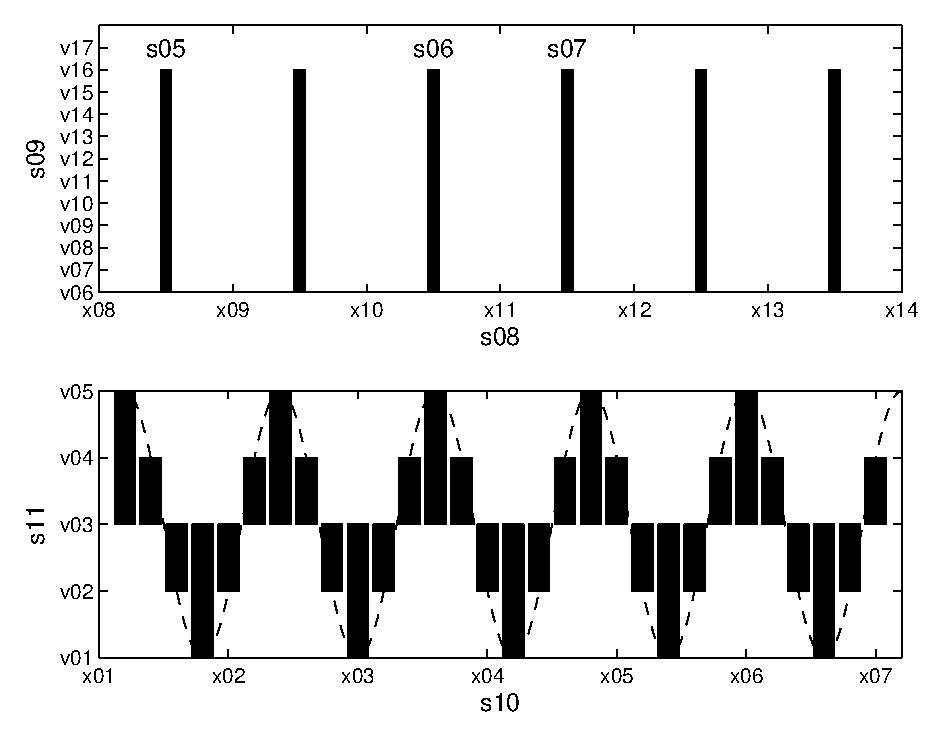
\includegraphics[width=0.9\textwidth]{figs/f_Qs_30_p_5_1.eps}}%
\end{psfrags}%
%
% End f_Qs_30_p_5_1.tex
\end{document}
% See http://www.mathworks.de/matlabcentral/fileexchange/loadFile.do?objectId=4638
% for recent versions of laprint.m.
%
% created by:           LaPrint version 3.16 (13.9.2004)
% created on:           12-Nov-2008 21:46:31
% eps bounding box:     17.5 cm x 13.125 cm
% comment:              
%
\begin{psfrags}%
\psfragscanon%
%
% text strings:
\psfrag{s05}[b][b]{$\xi_{5}$}%
\psfrag{s06}[b][b]{$\xi_{25}$}%
\psfrag{s07}[b][b]{$\xi_{35}$}%
\psfrag{s08}[t][t]{$\nu$}%
\psfrag{s09}[b][b]{$\xi_{\nu}$}%
\psfrag{s10}[t][t]{Slot number}%
\psfrag{s11}[b][b]{$F_{slot}/\SI{}{A}$}%
%
% xticklabels:
\psfrag{x01}[t][t]{0}%
\psfrag{x02}[t][t]{5}%
\psfrag{x03}[t][t]{10}%
\psfrag{x04}[t][t]{15}%
\psfrag{x05}[t][t]{20}%
\psfrag{x06}[t][t]{25}%
\psfrag{x07}[t][t]{30}%
\psfrag{x08}[t][t]{0}%
\psfrag{x09}[t][t]{10}%
\psfrag{x10}[t][t]{20}%
\psfrag{x11}[t][t]{30}%
\psfrag{x12}[t][t]{40}%
\psfrag{x13}[t][t]{50}%
\psfrag{x14}[t][t]{60}%
%
% yticklabels:
\psfrag{v01}[r][r]{-1}%
\psfrag{v02}[r][r]{-0.5}%
\psfrag{v03}[r][r]{0}%
\psfrag{v04}[r][r]{0.5}%
\psfrag{v05}[r][r]{1}%
\psfrag{v06}[r][r]{0}%
\psfrag{v07}[r][r]{0.1}%
\psfrag{v08}[r][r]{0.2}%
\psfrag{v09}[r][r]{0.3}%
\psfrag{v10}[r][r]{0.4}%
\psfrag{v11}[r][r]{0.5}%
\psfrag{v12}[r][r]{0.6}%
\psfrag{v13}[r][r]{0.7}%
\psfrag{v14}[r][r]{0.8}%
\psfrag{v15}[r][r]{0.9}%
\psfrag{v16}[r][r]{1}%
\psfrag{v17}[r][r]{1.1}%
%
% Figure:

\subfloat[Slot mmf and winding factors\label{fig:f_Qs30_5_1}]{%
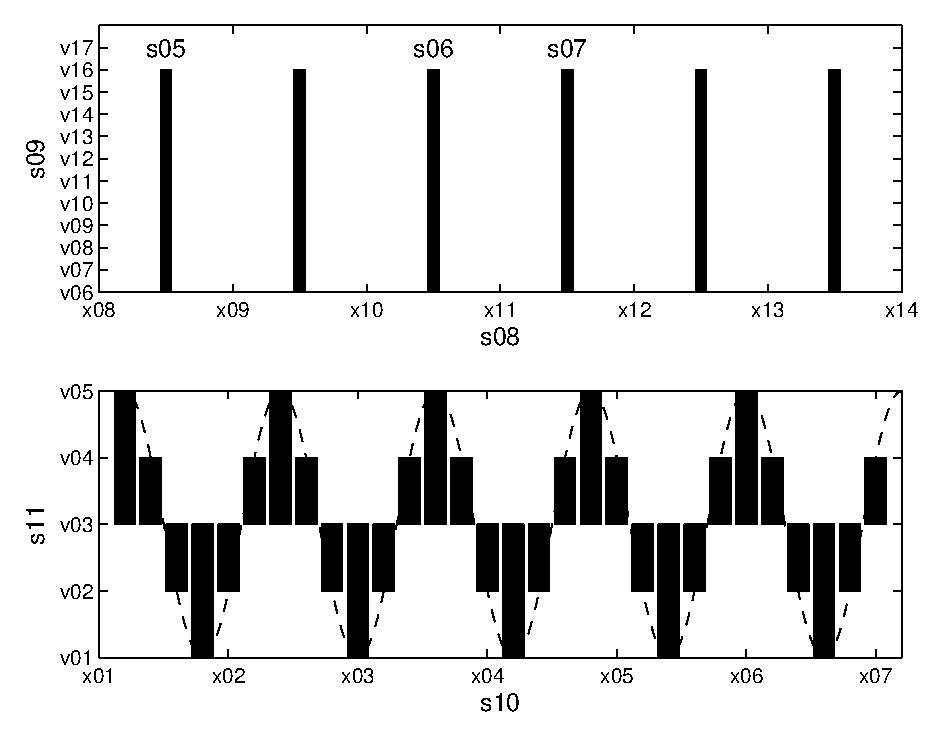
\includegraphics[width=0.9\textwidth]{figs/f_Qs_30_p_5_1.eps}}%
\end{psfrags}%
%
% End f_Qs_30_p_5_1.tex
\end{document}
% See http://www.mathworks.de/matlabcentral/fileexchange/loadFile.do?objectId=4638
% for recent versions of laprint.m.
%
% created by:           LaPrint version 3.16 (13.9.2004)
% created on:           12-Nov-2008 21:46:31
% eps bounding box:     17.5 cm x 13.125 cm
% comment:              
%
\begin{psfrags}%
\psfragscanon%
%
% text strings:
\psfrag{s05}[b][b]{$\xi_{5}$}%
\psfrag{s06}[b][b]{$\xi_{25}$}%
\psfrag{s07}[b][b]{$\xi_{35}$}%
\psfrag{s08}[t][t]{$\nu$}%
\psfrag{s09}[b][b]{$\xi_{\nu}$}%
\psfrag{s10}[t][t]{Slot number}%
\psfrag{s11}[b][b]{$F_{slot}/\SI{}{A}$}%
%
% xticklabels:
\psfrag{x01}[t][t]{0}%
\psfrag{x02}[t][t]{5}%
\psfrag{x03}[t][t]{10}%
\psfrag{x04}[t][t]{15}%
\psfrag{x05}[t][t]{20}%
\psfrag{x06}[t][t]{25}%
\psfrag{x07}[t][t]{30}%
\psfrag{x08}[t][t]{0}%
\psfrag{x09}[t][t]{10}%
\psfrag{x10}[t][t]{20}%
\psfrag{x11}[t][t]{30}%
\psfrag{x12}[t][t]{40}%
\psfrag{x13}[t][t]{50}%
\psfrag{x14}[t][t]{60}%
%
% yticklabels:
\psfrag{v01}[r][r]{-1}%
\psfrag{v02}[r][r]{-0.5}%
\psfrag{v03}[r][r]{0}%
\psfrag{v04}[r][r]{0.5}%
\psfrag{v05}[r][r]{1}%
\psfrag{v06}[r][r]{0}%
\psfrag{v07}[r][r]{0.1}%
\psfrag{v08}[r][r]{0.2}%
\psfrag{v09}[r][r]{0.3}%
\psfrag{v10}[r][r]{0.4}%
\psfrag{v11}[r][r]{0.5}%
\psfrag{v12}[r][r]{0.6}%
\psfrag{v13}[r][r]{0.7}%
\psfrag{v14}[r][r]{0.8}%
\psfrag{v15}[r][r]{0.9}%
\psfrag{v16}[r][r]{1}%
\psfrag{v17}[r][r]{1.1}%
%
% Figure:

\subfloat[Slot mmf and winding factors\label{fig:f_Qs30_5_1}]{%
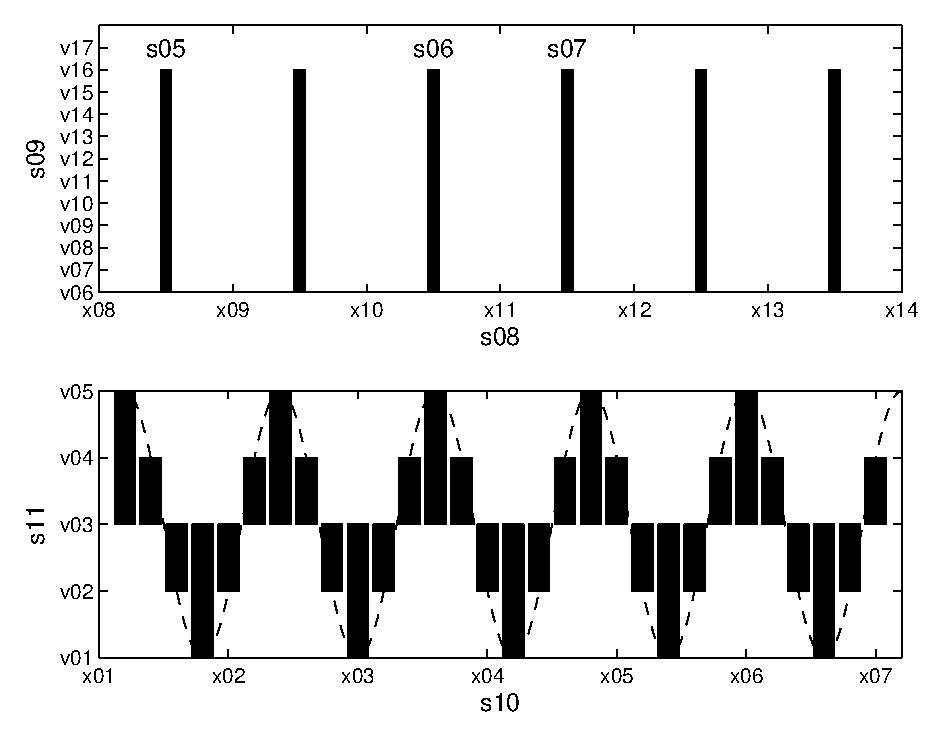
\includegraphics[width=0.9\textwidth]{figs/f_Qs_30_p_5_1.eps}}%
\end{psfrags}%
%
% End f_Qs_30_p_5_1.tex
